
% 绪论
\chapter{绪论}

\section{涵道式无人机的研究背景}
无人驾驶航空器（Unmanned Aerial Vehicle, UAV）的快速发展正在深刻重塑现代社会的生产生活方式。作为低空经济（Low-Altitude Economy）的核心载体，无人机凭借其灵活性、便捷性和可扩展性，在军事侦察、精准农业、工业巡检、城市物流等众多领域展现出巨大的应用潜力。旋翼无人机相较于固定翼飞行器，其垂直起降和悬停能力使其在执行定点、精准和详查任务时独具优势，填补了有人驾驶航空器在复杂环境下的作业空白。

近年来，低空经济作为战略性新兴产业，正加速从“飞起来”向“用起来”跃升。据预测，2025年我国低空经济市场规模将达到1.5万亿元，2030年有望突破2万亿元。在军事领域，无人机已成为现代战争中情报获取、目标监视乃至精确打击的关键装备；在农业领域，农用无人机突破地形与人力限制\cite{liaoyong}，让播种、植保、监测从地面延伸至低空；在工业领域，无人机广泛应用于电力巡检、油气管道监测、光伏面板清洁等作业场景，显著提升了运维效率；在运输领域，无人机物流正从试点走向常态——从城市上空的“分钟级配送”到山区乡村的“最后一公里”，低空物流正在改变传统物流格局，医疗样本的空中转运更成为守护生命的快速通道。2026年5月即将实施的《民用无人驾驶航空器实名登记和激活要求》与《民用无人驾驶航空器系统运行识别规范》，标志着我国无人机产业正从“野蛮生长”走向“规范提质”，为低空经济的健康可持续发展奠定了制度基础。

在农业领域，以大疆农业为代表的无人化作业模式正推动传统农业向智慧化转型。王冰洁等学者应用大疆T40型植保无人飞机对杧果树冠层进行喷雾作业研究，系统探究了雾滴粒径、作业高度、作业速度等参数对雾滴沉积分布的影响，为果园空中喷洒作业提供了理论指导和参数优化依据\cite{wangbingjie}。此外研究人员利用大疆M3M无人机采集春玉米秋耕农田的多光谱数据，结合机器学习算法构建土壤含水率反演模型，为农田墒情监测和智慧化灌溉提供了数据支撑\cite{fanzikang}。这些研究表明，农业无人机在精准施药、作物监测、变量施肥等环节的应用已从工程实践走向学术研究，其作业参数优化与控制方法正成为农业工程领域的重要研究方向。

在运输领域，无人机物流配送正从试点走向常态。美团无人机自2021年启动常态化运营以来，已在城市即时配送场景中积累了丰富的运行经验。美团机器人研究院与IDEA研究院联合研发的智能避障系统取得重要进展，通过云端视觉大模型升级，系统在识别风筝、气球、吊车等复杂空中目标时召回率显著提升，误检率大幅下降，相关成果已在公园等复杂配送场景中实现应用。

\begin{figure}[htbp]
    \centering
    \begin{minipage}[b]{0.45\textwidth}
        \centering
        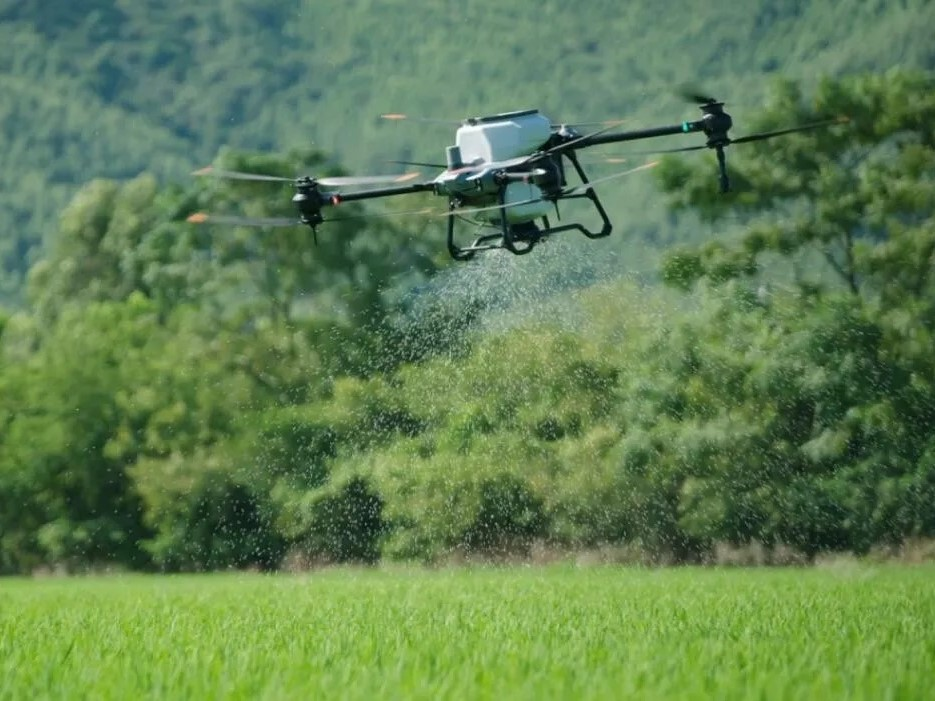
\includegraphics[width=\textwidth]{figure/DJI_T40.jpeg}
        \caption{\label{fig:DJI_T40}大疆T40植保无人机}
    \end{minipage}
    \hfill  % 产生弹性水平间距
    \begin{minipage}[b]{0.45\textwidth}
        \centering
        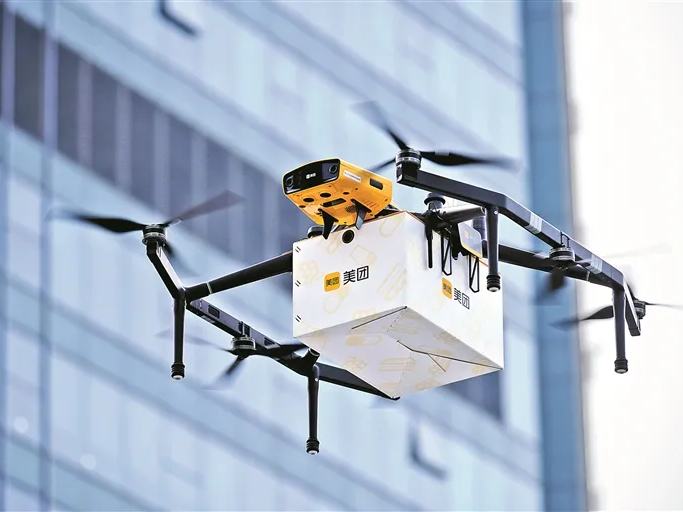
\includegraphics[width=\textwidth]{figure/meituanUAV.png}
        \caption{\label{fig:meituanUAV}美团运输无人机}
    \end{minipage}
\end{figure}

在军事领域，无人机已成为现代战争中情报获取、目标监视乃至精确打击的关键装备。从俄乌冲突的实战经验来看，无人机已发展成为战役战术体系中的核心作战力量，形成察打一体与蜂群战术相结合的立体作战模式，这种"发现即摧毁"的非接触打击方式正在动摇机械化战争时代形成的传统陆战理论。具体到装备层面，察打一体无人机的型号谱系不断丰富。以TB-001"双尾蝎" 为代表的察打一体无人机，采用螺旋桨动力，最大起飞重量近3吨，有效载荷超1吨，最大航程可达6000公里，可携带包括空地导弹、精确制导炸弹在内的16枚空地打击弹药，具备全天候侦察能力和"看到即打到"的察打一体能力。在2018年的中国航展上，具备全天候作战能力和复杂环境适应能力的BZK-005E首次亮相，它可配备光电吊舱、合成孔径雷达和通信、电子对抗等各类载荷，用于执行战役级情报、监视、侦察和打击任务，其载荷能力可达数百公斤，堪称"一机多能"\cite{BZK-005E}。随着战争形态加速演变，无人机以其低成本，高机动性和隐蔽性，正在逐渐成为国防军事中不可或缺的中坚力量。

\begin{figure}[htbp]
    \centering
    \begin{minipage}[b]{0.45\textwidth}
        \centering
        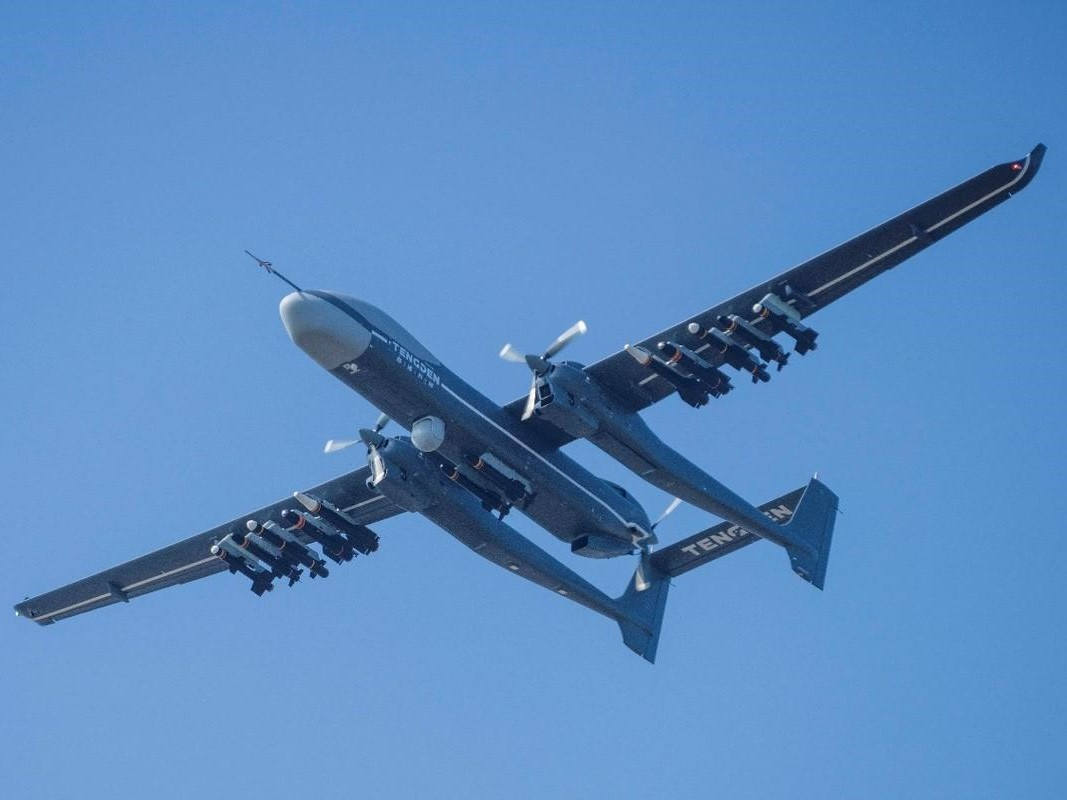
\includegraphics[width=\textwidth]{figure/shuangweixie.jpg}
        \caption{TB-001"双尾蝎"无人机}
    \end{minipage}
    \hfill  % 产生弹性水平间距
    \begin{minipage}[b]{0.45\textwidth}
        \centering
        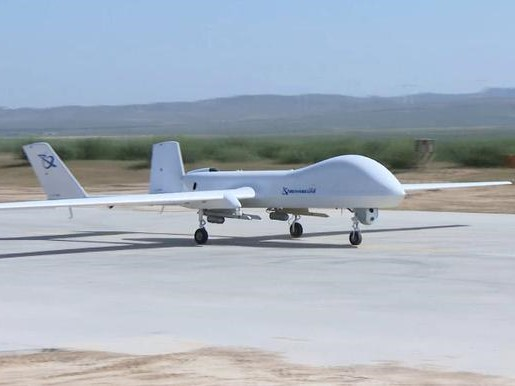
\includegraphics[width=\textwidth]{figure/BKZ_005E.jpg}
        \caption{\label{fig:BKZ-005E}BKZ-005E无人机}
    \end{minipage}
\end{figure}

在赈灾救援领域，无人机凭借其快速响应、灵活部署和环境适应性强等优势，正成为自然灾害应急救援体系中不可或缺的关键装备。El-Sakka等学者指出，无人机在人道主义救援中可显著缩短关键物资的配送时间，为危机决策提供实时数据支持，在自然灾难、冲突区域和健康危机等场景中展现出灵活、高效、成本可控的显著优势\cite{El-Sakka}。


在众多无人机技术路线中，涵道式无人机（Ducted Fan UAV）因其独特的结构设计和优异的气动性能，日益受到学术界和工业界的广泛关注\cite{renxiaolu}\cite{xuchang}。涵道风扇（Ducted Fan）是指在螺旋桨风扇外围设置涵道（导管）的一种推进装置，其工作原理与孤立螺旋桨有本质区别。

从结构特点来看，涵道式无人机可根据姿态控制方式与扭矩平衡机制划分为不同类型。常见的结构形式包括单旋翼结构和共轴双旋翼结构。单旋翼结构通常采用环形涵道设计，动力系统安装于涵道中央，通过固定翼板稳定于涵道内部，并由控制翼板（导流片）实现姿态控制\cite{lijianbo}；共轴双旋翼结构则通过等速对转的双旋翼平衡反扭矩，采用旋转倾斜器改变旋翼周期变距以控制飞行器姿态。此外，还有倾转涵道、多涵道组合等构型，以满足不同应用场景的需求。

涵道式无人机气动性能的优越性源于其独特的流动机理。与孤立螺旋桨相比，涵道的存在从根本上改变了风扇的气动工作环境：一方面，涵道有效限制了叶尖涡流的形成和发展，减少了叶尖处的诱导阻力与冲击噪声，从而降低能量损失；另一方面，涵道入口处的唇口可产生附加升力，研究表明小型涵道风扇可提供高达20\%的附加升力，使涵道风扇在相同功率消耗下能够产生比孤立螺旋桨更大的推力。涵道对气动噪声具有良好的屏蔽作用，使整机噪声水平显著降低\cite{lijianbo}。

涵道式无人机具备以下几方面突出优势：

第一，安全性高。涵道将旋翼完全或大部分环括于内部，能有效避免裸露旋翼割伤人员和碰撞障碍物的事故发生。这一特性使涵道式无人机特别适合在狭小空间、近人环境以及城市复杂地形中作业。例如，以色列Urban Aeronautics公司开发的Cormorant（又称AirMule）无人机，采用涵道风扇技术，可在建筑物密集区域、陡峭山地等传统直升机难以进入的环境执行搜救和物资投送任务，其旋翼内置设计不仅提高了安全性，也显著降低了气动噪声。中国航天科工二院研发的微小型涵道风扇无人机，外表采用柔软发泡材料包裹，进一步提升了防撞性能，完全满足近地/近人场景的安全需求。

第二，气动效率高。涵道的存在改变了风扇的气动工作环境：一方面，涵道限制了叶尖涡流的形成和发展，减少了诱导阻力，从而降低能量损失；另一方面，涵道入口的合理设计可改善进气条件。研究表明，与同等直径的孤立螺旋桨相比，涵道风扇能够产生更高的推力性能、更高的推进效率和更低的噪声特性\cite{Numerical_and_Experimental_Analyses_of_the_Ducted_Fan}。通过将螺旋桨封闭在涵道内，不仅可以降低裸露旋翼带来的风险，还能通过减小叶尖损失和优化气流组织来改善气动性能\cite{Aerodynamic_performance_assessment_of_a_ducted_fan_UAV}。近期研究还表明，针对边界层吸入（Boundary Layer Ingestion, BLI）进气条件，通过在涵道唇口设计鼓包等流动控制方法，可有效改善进气畸变，降低气动损失\cite{wangshuo}。

第三，具备垂直起降能力且结构紧凑。涵道式无人机继承了旋翼飞行器垂直起降和悬停的优点\cite{Xia}，能够在无跑道条件下起降，适用于舰载、山地、城市峡谷等复杂环境。这类飞行器继承了旋翼飞行器垂直起降和悬停的优点，能够在无跑道条件下起降，适用于舰载、山地、城市峡谷等复杂环境。同时，涵道结构使整机布局更为紧凑，体积小巧，便于携带和收纳。

涵道式无人机以其安全可靠、气动高效、垂直起降和结构紧凑等综合优势，正成为无人机技术研究的重要方向之一。随着低空经济应用场景的持续拓展，涵道式无人机在人员搜救、复杂环境侦查、管道巡检、城市空中交通等领域的应用前景将更加广阔。深入开展涵道式无人机气动设计、飞行控制与系统集成研究，对于推动我国无人机技术自主创新、抢占低空经济制高点具有重要的理论意义和工程价值。

\section{涵道式无人机的研究历史和现状}
涵道风扇的空气动力学概念可追溯至20世纪30年代。1936年，罗马尼亚发明家亨利·科安达（Henri Coandă）在其专利中首次描述了利用附着效应改变气流方向的方法\cite{coanda1938propelling}。同一时期，意大利工程师路易吉·斯蒂帕（Luigi Stipa）对"内嵌螺旋桨"的涵道机身进行了风洞实验，发现这种构型能显著提升螺旋桨的静推力效率\cite{stipa1932experiments}。1936年，德国工程师路德维希·科特（Ludwig Kort）在美国申请了船舶螺旋桨的涵道装置专利，这被认为是现代涵道推进器的雏形\cite{kort1936combined}。

第二次世界大战后，随着空气动力学理论的发展和喷气式飞机的兴起，涵道风扇作为一种潜在的垂直起降（VTOL）动力方案受到更多关注。1940年代，德国AVA研究所的克吕格（Krüger）对不同形状的涵道剖面进行了系统性的实验研究，探讨了扩压器角度、入口唇口半径等参数对性能的影响\cite{kruger1949wind}。此后，库赫曼（Küchemann）和韦伯（Weber）在英国开展了涵道螺旋桨的理论分析工作，奠定了涵道风扇气动设计的基础\cite{kuechemann1953aerodynamics}。

在工程应用层面，1950年代至1960年代成为涵道风扇垂直起降飞行器发展的黄金时期。美国在这一时期研制了多种基于涵道风扇的飞行平台，包括希勒（Hiller）VZ-1“波尼”、皮亚塞茨基（Piasecki）VZ-8“空中吉普”、多克（Doak）VZ-4等\cite{parlett1955aerodynamic}。这些机型均采用涵道风扇作为主要升力装置，试图实现兼具直升机垂直起降能力和固定翼飞机高速巡航能力的飞行器。然而受限于当时的技术水平，这些项目大多停留在验证机阶段，未能投入实际应用。
\begin{figure}[htbp]
    \centering
    \begin{minipage}[b]{0.45\textwidth}
        \centering
        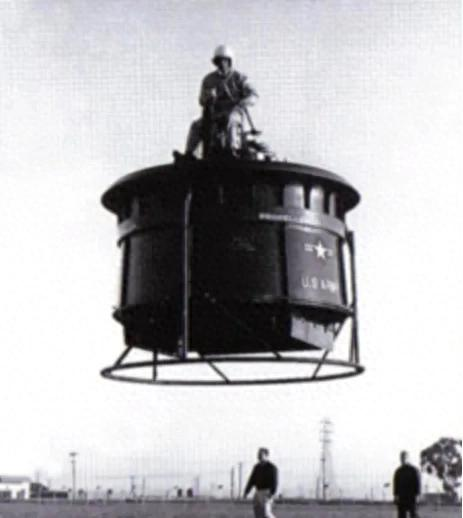
\includegraphics[height=0.22\textheight]{figure/Hiller VZ-1.jpeg}
        \caption{希勒（Hiller）VZ-1}
    \end{minipage}
    \hfill  % 产生弹性水平间距
    \begin{minipage}[b]{0.45\textwidth}
        \centering
        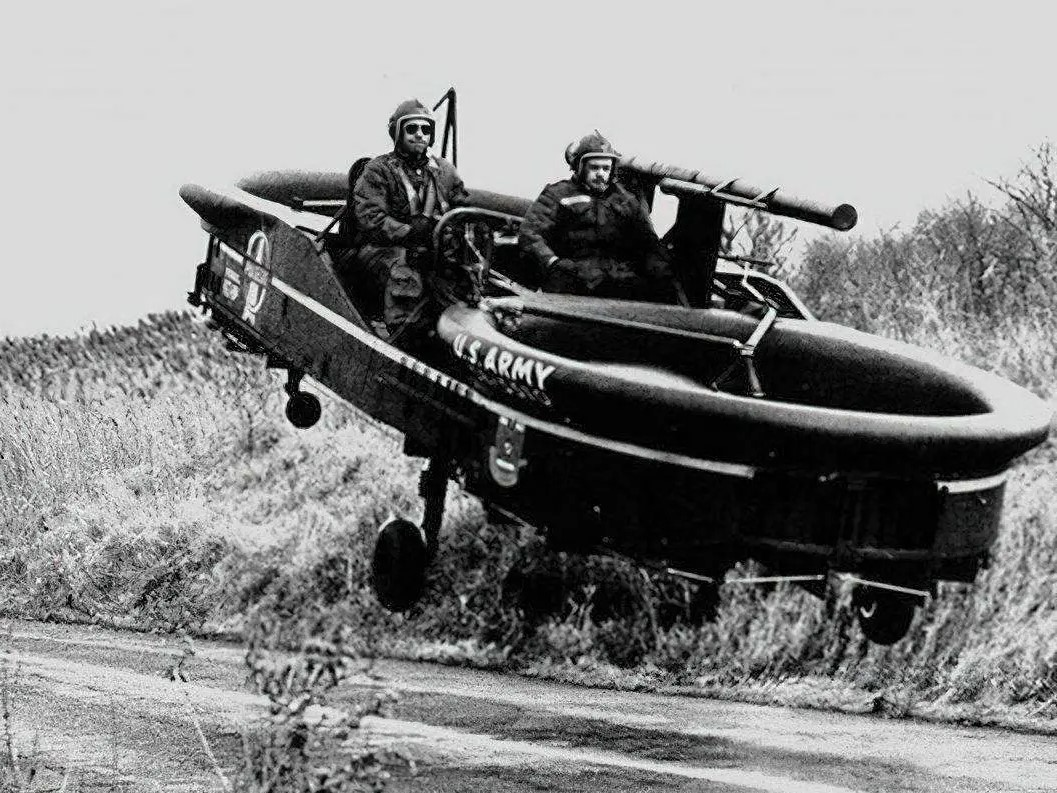
\includegraphics[height=0.22\textheight]{figure/Piasecki VZ-8.jpg}
        \caption{皮亚塞茨基（Piasecki）VZ-8}
    \end{minipage}
\end{figure}

值得注意的是，同一时期还出现了涵道风扇的另一种重要应用——直升机涵道尾桨。1970年，法国宇航公司（Aérospatiale）在SA.341“小羚羊”直升机上首次采用了称为“芬尼斯特龙”（Fenestron）的涵道尾桨设计\cite{mouille1970fenestron}。这种将尾桨置于涵道内的构型不仅提高了安全性，还降低了噪声，成为涵道风扇技术在航空领域的首次成功商业化应用。此后，欧洲直升机公司（Eurocopter，现空客直升机）在多款机型中持续发展这一技术\cite{vuillet1986new}。
\begin{figure}[htbp]
    \centering
    \begin{minipage}[b]{0.45\textwidth}
        \centering
        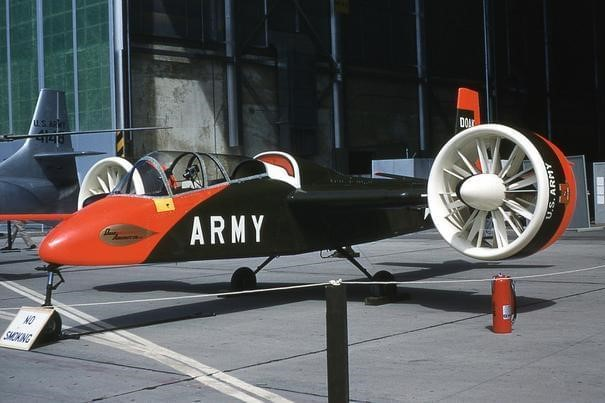
\includegraphics[height=0.2\textheight]{figure/Doak VZ-4.jpg}
        \caption{多克（Doak）VZ-4}
    \end{minipage}
    \hfill  % 产生弹性水平间距
    \begin{minipage}[b]{0.45\textwidth}
        \centering
        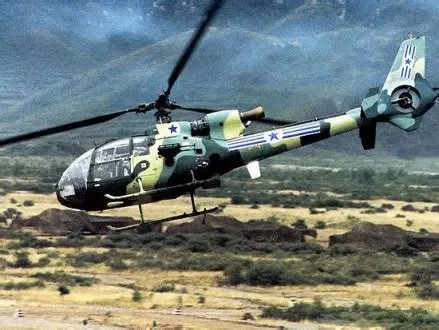
\includegraphics[height=0.2\textheight]{figure/SA.341.jpg}
        \caption{SA.341“小羚羊”直升机}
    \end{minipage}
\end{figure}


1980年代，随着微电子技术、传感器技术和控制理论的发展，无人机开始从军事靶机向具有任务能力的侦察平台演进。涵道风扇构型因其结构紧凑、安全性高的特点，被多个研究机构选为新型垂直起降无人机的技术方案。

美国海军研究实验室于1986年启动了“地面空中遥操作系统”（GATERS）项目，其中涵道式飞行器AROD（Airborne Remotely Operated Device）是该系统的空中观测组件\cite{spawar1999arod}。AROD采用单发涵道风扇设计，通过光纤传输控制信号和图像数据，实现了垂直起降和空中悬停。尽管受限于当时的动力和航电技术，AROD的续航能力和载荷水平有限，但它验证了涵道式无人机用于战场侦察的可行性\cite{murphy1995lookout}。

1990年代，西科斯基飞机公司（Sikorsky Aircraft）以自筹资金开发了Cypher涵道式无人机\cite{cycon1992sikorsky}。Cypher采用同轴双旋翼涵道构型，通过旋翼的周期变距和总距控制实现六自由度运动，无需额外的控制舵面。该机于1993年完成首次自主起降，1998年实现了悬停、前飞和垂直/水平模态转换的全自主飞行\cite{walsh1998sikorsky}。Cypher的技术验证为后续涵道式无人机的发展积累了宝贵经验。

\begin{figure}[htbp]
    \centering
    \begin{minipage}[b]{0.45\textwidth}
        \centering
        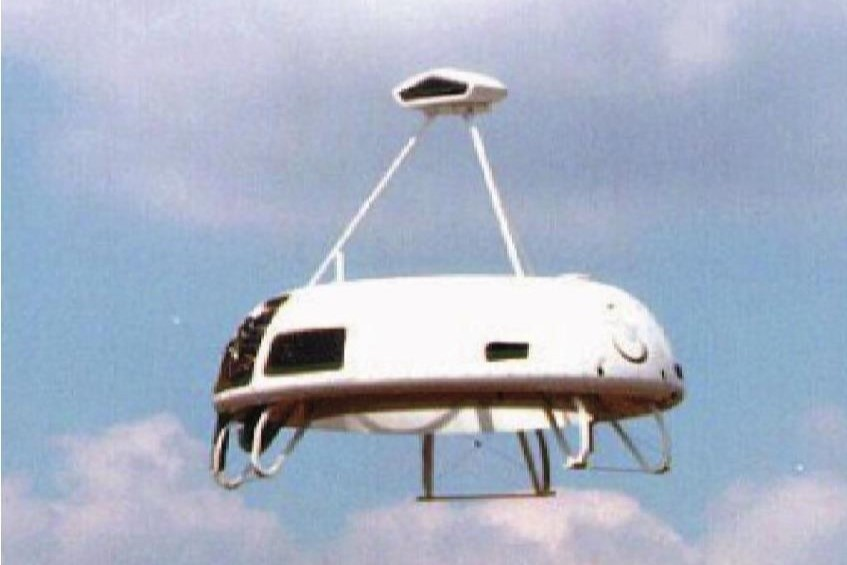
\includegraphics[width=\textwidth]{figure/cypher.jpg}
        \caption{Cypher涵道式无人机}
    \end{minipage}
    \hfill  % 产生弹性水平间距
    \begin{minipage}[b]{0.45\textwidth}
        \centering
        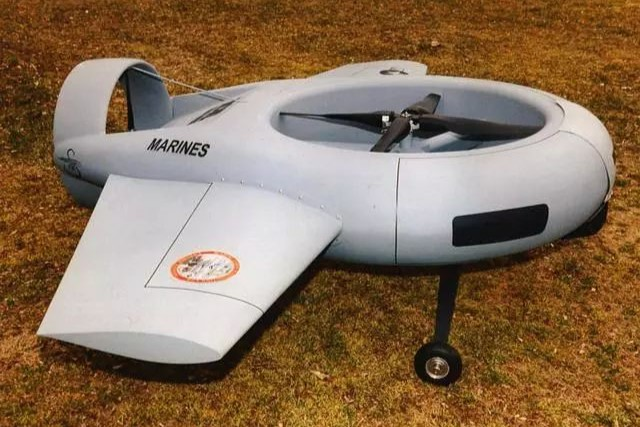
\includegraphics[width=\textwidth]{figure/cypherII.jpg}
        \caption{Cypher II涵道式无人机}
    \end{minipage}
\end{figure}


与此同时，桑迪亚国家实验室（Sandia National Laboratories）与MLB公司合作开发了另一种构型的涵道式无人机。该方案采用单旋翼加固定导叶和控制舵面的设计，通过舵面偏转产生姿态控制力矩。这种构型结构简单、成本较低，为后续多种涵道式无人机提供了技术原型\cite{weir1988aerodynamic}。

尽管涵道风扇作为独立升力装置能够实现垂直起降，但其巡航效率远低于常规固定翼飞机。为解决这一问题，研究人员开始探索将涵道风扇与固定翼相结合的混合构型，即涵道式垂直起降固定翼无人机（Ducted Fan Tailsitter VTOL）\cite{cheng2022phd}。

2003年，美国极光飞行科学公司（Aurora Flight Sciences）为DARPA的OAV-II项目研制了GoldenEye系列涵道式无人机\cite{schaefer2003goldeneye}。GoldenEye-50机身长70cm，翼展1.4m，采用尾推式涵道风扇作为单一动力源。在垂直起降阶段，涵道风扇提供升力；转入水平飞行后，机翼产生升力，涵道风扇改为提供前飞推力。这种构型不仅保留了涵道风扇的安全特性，还大幅提升了巡航效率和航时。

韩国科学技术院（KAIST）的郑延德（Yeunduk Jung）等人于2013年报道了一款小型涵道式尾座无人机\cite{jung2012development}。该机翼展1.3m，起飞重量2.9kg，采用多模态切换控制器实现了垂直起降、过渡飞行和水平巡航的完整飞行试验。

涵道式尾座无人机发展的重要里程碑是美国马丁无人机公司（Martin UAV）的V-bat系列。该机型最早由MLB公司于2008年开始研发，2015年后由马丁无人机公司持续推进\cite{yang2019vbat}。V-bat起飞重量37.2kg，翼展2.75m，最大航时达8小时，采用一台Hirth 4201活塞发动机驱动涵道风扇。该机于2017年完成了舰上起降试验，2018年在山地和丛林环境中进行了飞行演示，是目前最为成熟的涵道式尾座无人机系统。阿盖尔（Argyle）等人在其博士论文中详细阐述了V-bat的建模与控制方法\cite{argyle2016modeling}。

\begin{figure}[htbp]
    \centering
    \begin{minipage}[b]{0.45\textwidth}
        \centering
        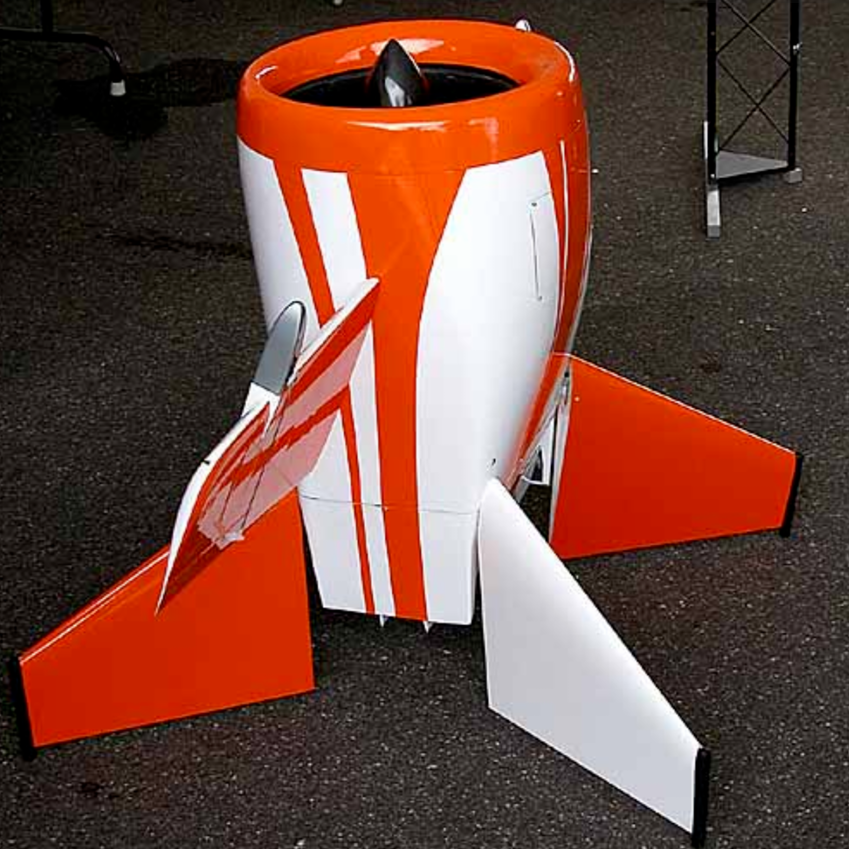
\includegraphics[height=0.2\textheight]{figure/golden_eye.png}
        \caption{GoldenEye涵道式无人机}
    \end{minipage}
    \hfill  % 产生弹性水平间距
    \begin{minipage}[b]{0.45\textwidth}
        \centering
        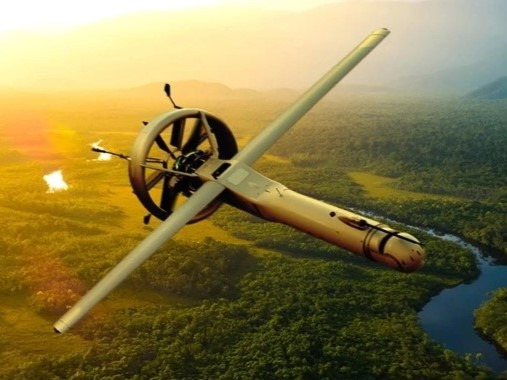
\includegraphics[height=0.2\textheight]{figure/v-bat.jpg}
        \caption{V-bat涵道式无人机}
    \end{minipage}
\end{figure}

\subsection{涵道式无人机的地面效应}
地面效应（Ground Effect, GE）是指当飞行器在接近地面或其它刚性表面运行时，由于地面的存在改变了气流分布，从而导致气动特性发生显著变化的现象\cite{matuz2021ground}。对于涵道式无人机而言，地面效应主要体现在垂直起降、悬停和低空飞行等阶段。由于涵道式无人机的地面效应产生原因较为复杂，并且各个研究团队的实验对象不一致，目前研究涵道式无人机的地面效应的常见方式是试验分析和CFD仿真，尚且不存在一种普适性的方式能够计算出一般涵道无人机在近地面受到的扰动。

美国NASA团队对涵道风扇的地面效应的研究起步较早，在20世纪60年代，针对涵道螺旋桨在倾转涵道垂直起降飞行器上的应用，进行了一系列风洞试验研究，为后续学者研究地面效应的机理提供宝贵的基础试验数据库\cite{yaggy1961aerodynamics}\cite{yaggy1961wind}。Jardin等研究了微小型旋翼在受限环境中的气动性能，发现靠近地面时产生的湍流涡流和脉动速度会影响涵道螺旋桨的稳定性\cite{jardin2017aerodynamic}。Prothin等研究了MAV旋翼在地面和角落效应中的空气动力学特性\cite{prothin2019aerodynamics}。随着CFD技术的发展，Graber、Itoga等学者开发了多种数值方法模拟近地旋翼流场，该方法提高了分析无人机地面效应的效率，但多数研究聚焦于开放式旋翼\cite{graber1990investigation}。

西北工业大学研究团队建立了涵道螺旋桨地面效应试验与数值计算相结合的研究方法，通过地面台架试验和基于滑移网格技术的CFD仿真，系统研究了不同近地高度下的涵道螺旋桨拉力和功率特性\cite{deng2020ground}。揭示了地面效应的影响机理：地面形成阻滞涵道出口喷流的高压区和向上的反弹气流，高压区使螺旋桨拉力增大，而反弹涡环吸入唇口后减小涵道拉力\cite{Aerodynamic_performance_assessment_of_a_ducted_fan_UAV}。北京理工大学研究团队针对新型共轴涵道风扇飞行机器人，开展了地面效应下的气动分析与控制研究，并通过涵道风扇台架试验，获得了不同高度下地面效应推力的拟合曲线\cite{ai2020aerodynamic}。他们采用CFD软件分析了不同高度下原型机的流场特性，发现随高度降低，下洗流偏转增大，有效流通面积减小，形成地面涡和桨尖涡\cite{fan2022novel}。清华大学研究团队采用URANS方法和滑移网格技术，研究了地面效应对涵道风扇非定常特性的影响。时均结果表明，地面导致涵道推力下降、桨叶推力增加、总推力降低。瞬态结果表明，在地面效应下会出现具有周向运动的小尺度失速涡胞\cite{luo2023numerical}。南京航空航天大学研究团队对涵道风扇空气动力学特性进行了系统分析，研究了涵道风扇与孤立螺旋桨的性能差异\cite{li2005aerodynamic}。开展了涵道风扇升力系统的升阻特性试验研究，发现前飞时涵道阻力较大，涵道风扇若作为升力装置仅适用于强调悬停和低速飞行性能的飞行器\cite{li2004experimental}。

为实现无人机在近地面的鲁棒控制，科研人员在已有的无人机控制器的基础上，针对地面效应带来的扰动设计了相对应的控制策略。北京理工大学团队设计了非线性扰动观测器（NDO）结合双闭环PID控制结构，用于补偿地面效应产生的扰动力。仿真和实验结果表明，该控制结构使高度跟踪误差从6cm减小到1.8cm，能有效补偿大部分地面效应扰动\cite{ai2020aerodynamic}。

\subsection{涵道式无人机的飞行控制}
对于任何无人机而言，飞行控制技术都是其核心设计环节之一，飞行控制直接影响着无人机的核心性能。学者们普遍认识到，精确的动力学模型是控制设计的基础，然而涵道无人机的模型远比常规旋翼机复杂。

在早期，由于对涵道风扇的独特气动特性认识不足，涵道式无人机的常见控制方法是线性控制技术。此外，线性控制技术的设计简单，计算量小的优势。李远伟等在涵道式无人机的姿态控制中设计了基于PID的控制系统，并在飞行试验中验证了其在悬停和小角度机动下的姿态跟踪能力\cite{li2010robust}。然而，PID控制在面对大攻角前飞、强风扰或参数变化时，鲁棒性较差，容易出现跟踪误差或失稳现象。Pflimlin等也在HoverEye无人机的姿态控制中采用了PID结构，用于底层姿态稳定，但指出该方法在面对复杂气动环境时存在局限性，需结合更高级的控制策略进行补偿\cite{pflimlin2007position}。线性二次型调节器（LQR）及其扩展形式——线性二次型跟踪器（LQT）和带有积分器的线性二次型跟踪器（LQTI），在处理多输入多输出（MIMO）系统的耦合问题时具有天然优势。Jeong等针对韩国忠南大学的涵道式无人机，设计了基于LQTI的控制系统，覆盖悬停、过渡和巡航三种飞行模式\cite{jeong2015control}。通过在状态向量中引入积分项，显著降低了稳态误差，并在风扰环境下进行了三维修航点导航仿真，验证了其在全飞行包线内的控制效果。H∞控制理论因其能够显式处理模型不确定性和外部扰动，成为涵道式无人机控制设计中广泛采用的鲁棒控制方法。李远伟等针对涵道式无人机在参数摄动和风扰下的姿态控制问题，设计了基于H∞理论的鲁棒控制器。通过线性矩阵不等式（LMI）求解，实现了对模型不确定性和外部扰动的有效抑制。仿真与飞行试验表明，相比PID控制，H∞控制器在姿态跟踪精度、噪声抑制和参数变化下的鲁棒性方面均表现更优\cite{li2010robust}。Fan等针对一种新型双涵道无人机，设计了基于H∞综合的结构化多回路姿态控制器，并采用非光滑优化方法进行参数整定。该控制器在内环实现静态输出反馈稳定，外环用于姿态跟踪。仿真与飞行实验验证了其在强耦合和非线性条件下的良好控制性能\cite{fan2018modelling}。

由于线性控制技术在某些特定场合的性能不尽人意，例如在大倾角飞行场景，近地面飞行场景和侧风场景科研人员开始探索非线性控制器以解决相关问题。Pflimlin等针对HoverEye无人机在未知侧风中的位置控制问题，提出了一种基于backstepping的自适应控制策略，将气动效应视为未知扰动进行在线估计。尽管控制器设计基于非线性理论，但其最终实现中仍保留了线性反馈结构，如对角速度的线性反馈控制，使得系统在工程应用中更易于实现\cite{pflimlin2007position}。滑模控制因其对匹配扰动的不变性而广泛应用于抗扰控制中，如文献\cite{manzoor2022composite}将滑模控制与扩张状态观测器结合，提升了系统对建模误差和风扰的鲁棒性。反步控制通过递归构造Lyapunov函数，适用于严反馈形式的系统，文献\cite{ai2025robust}将其应用于共轴双旋翼涵道无人机，实现了良好的姿态跟踪性能。自抗扰控制由韩京清提出，通过扩张状态观测器实时估计并补偿总扰动，已在涵道无人机中取得良好效果\cite{chen2024ADRC}。模型预测控制则因其处理约束的能力而受到重视，文献\cite{Manzoor2020VTOL, manzoor2022composite}将MPC与扰动观测器结合，实现了涵道无人机在全飞行模式下的轨迹跟踪控制。此外，动态逆方法因其能够直接对消系统非线性而成为研究热点\cite{zhu1997NDI, zhang2015NDI}。

非线性动态逆控制是一种基于反馈线性化的控制方法，其基本思想是通过对系统模型求逆，构造一个伪线性系统，从而简化控制器设计\cite{zhu1997NDI}。对于涵道无人机这类非线性系统，NDI能够实现对姿态和轨迹的精确跟踪，但其性能高度依赖于模型的准确性，对建模误差和外部扰动较为敏感\cite{zhang2015NDI}。为增强鲁棒性，研究者提出了增量非线性动态逆控制。INDI通过引入状态导数的反馈，将控制律构建为增量形式，显著降低了对系统模型的依赖，具有较强的抗扰能力\cite{wang2019flexible, smeur2016adaptive}。INDI已在多种飞行器上得到验证，如文献\cite{ludena2020flight}将其与平滑估计算法结合，实现了对战斗机的高精度姿态控制；文献\cite{Cheng2024INDI}将其应用于双涵道无人机，成功应对了地效干扰下的姿态控制问题。

尽管INDI在鲁棒性方面具有优势，但其控制性能仍受限于对状态导数估计的精度和延迟\cite{SteffensenINDI}。相比之下，NDI控制器在模型精确已知的情况下，能够实现更快的动态响应和更高的控制精度。文献指出，当执行器带宽足够高时，INDI可视为NDI在高频近似下的特例，但在低带宽执行器或强非线性条件下，NDI的优势更为明显\cite{SteffensenINDI}。此外，NDI框架更便于与参考模型结合，提供明确的误差动态设计，适用于对控制品质要求较高的任务场景。

综上所述，涵道无人机的非线性控制仍面临建模误差、外部扰动和执行器动态等多重挑战。本文将在现有研究基础上，针对地面效应带来的扰动和模型变化，围绕NDI与INDI控制器的设计与对比展开深入分析，结合扰动观测与状态估计技术，旨在提升涵道无人机在近地面端的控制性能与鲁棒性。


\subsection{涵道式无人机的气动参数辨识}


\section{本文的主要内容以及章节安排}
第一章为绪论，介绍了涵道式无人机的研究背景和意义，简要描述涵道式无人机在国内外的研究现状，并且总结了涵道式无人机的地面效应研究现状。最后介绍本文的主要内容及章节安排。第二章介绍本文的实验对象，描述涵道式无人机的运动学和动力学建模，定义本文使用的相关符号。为了观测本文使用的涵道式无人机在近地面处受到的扰动，第三章设计了一个实验用于测试在不同高度下的涵道螺旋桨推力和控制舵效，并且将实验数据可视化地呈现出来。第四章针对该地面效应带来的扰动，设计了一个抗扰动控制器，并通过实验证明该控制器的有效性。第五章设计了一种卡尔曼滤波器，能够实现在线测量涵道式无人机的各个气动参数，并且通过数值仿真和实飞测试的方式验证其有效性。最后是总结与展望。首先对全文的主要工作和结论进行系统性的总结，然后分析本文研究的不足之处，并根据不足对未来的研究工作进行展望。

\section{课题来源}
本课题研究来源于华南理工大学自动化科学与工程学院“自主系统与网络控制”教育部重点实验室的项目。项目支持基金：国家重点研发计划资助[2023YFB4704900]、航空科学基金项目资助[20220056060001]、国家自然科学基金重大科研仪器研制项目[61527810]、中国高校产学研创新基金新一代信息技术创新项目[2022IT046]、中央高校基本科研业务费专项资金资助。

\begin{figure}
    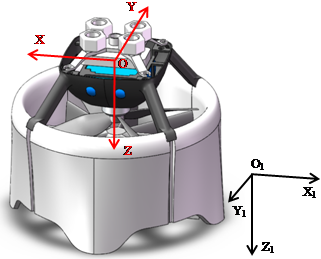
\includegraphics[scale=0.5]{figure/body1.png}
    \caption{\label{fig:aircraft}涵道式无人机结构图}
\end{figure}
